\documentclass[journal,12pt,twocolumn]{article}
\usepackage{graphicx}
\usepackage[none]{hyphenat}
\usepackage[margin=0.5in]{geometry}
\usepackage[cmex10]{amsmath}
\usepackage{array}
\usepackage{booktabs}
\usepackage{gensymb}
\usepackage{textcomp}
\title{\textbf{Circle Assignment}}
\author{Manideep Parusha - FWC22004}
\date{\today}

\providecommand{\norm}[1]{\left\lVert#1\right\rVert}
\providecommand{\abs}[1]{\left\vert#1\right\vert}
\let\vec\mathbf
\newcommand{\myvec}[1]{\ensuremath{\begin{pmatrix}#1\end{pmatrix}}}
\newcommand{\mydet}[1]{\ensuremath{\begin{vmatrix}#1\end{vmatrix}}}
\providecommand{\brak}[1]{\ensuremath{\left(#1\right)}}

\begin{document}

\maketitle
\section*{Problem}
\paragraph{Show that the tangents of circle drawn at the ends of diameter are parallel.}

\section*{Solution}

\begin{figure}[h]
\centering
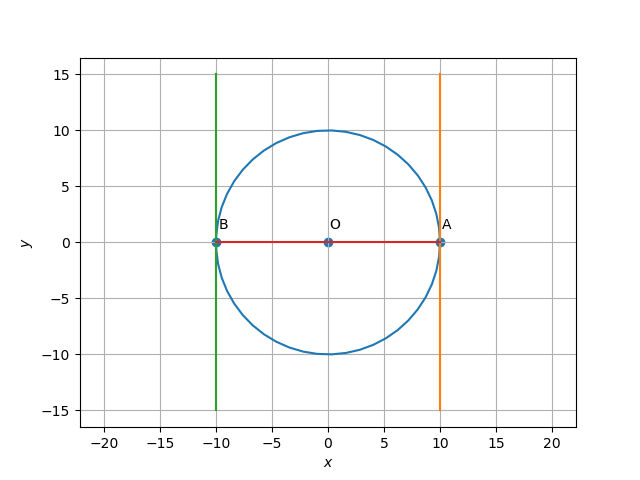
\includegraphics[width=\columnwidth]{figs/plot_cir.png}
\caption{Circle with tangents at ends of it's diameter}
\label{fig:cir_py}
\end{figure}

\subsection*{Construction}
Input taken for the construction of the Circle and the tangents is 'r' radius of the circle.

\begin{table}[h]
	\centering
\setlength\extrarowheight{2pt}
	\begin{tabular}{|c|c|c|}
		\hline
		\textbf{Symbol} & \textbf{Value} & \textbf{Description} \\
		\hline
		r & 10 & circle radius\\
		\hline
		O & (0,0,0) & Center\\
		\hline
		A & $(rcos(\theta),rsin(\theta),0)$ & point A\\
		\hline
		B & $(-rcos(\theta),-rsin(\theta),0)$ & point B\\
		\hline
	\end{tabular}
\end{table}

Let us assume a circle with radius 'r' and center at origin.\\
\begin{align}
	\boldsymbol{x}^{T}\boldsymbol{Vx} + 2\boldsymbol{u}^{T}x + f = 0
\end{align}
but, for a Circle 
\begin{align}
	\boldsymbol{V} = \myvec{ 1 & 0 & 0\\0 & 1&0\\0&0&1}
\end{align}
and the center of the circle is at origin,
\begin{align}
	\boldsymbol{u}^{T} = \myvec{ 0 \\0 \\0}
\end{align}
Here, the points \boldsymbol{A} and \boldsymbol{B} are the ends of diameter of the circle.\\
To prove that tangets at the ends of a diameter are parallel, we need to find the slope of tangents at the given points.

\begin{eqnarray}
	\vec{A} = \myvec{r.cos\theta \\r.sin\theta\\ 0},
	\vec{B} = \myvec{-r.cos\theta \\-r.sin\theta\\0}
\end{eqnarray}

We know that the cross product of two vectors results in a perpendicular vector, so we can find the tanget by cross multiplying radius vector and z-axisunit vector.

\begin{align}
	\vec{Z} = \myvec{0\\0\\1}
\end{align}
So, the tangents at \boldsymbol{A} and \boldsymbol{B} are given by,

\begin{align}
	\boldsymbol{T_1}= \boldsymbol{A} X \boldsymbol{Z},
	\boldsymbol{T_2} = \boldsymbol{B} X \boldsymbol{Z}
\end{align}
where \boldsymbol{A} and \boldsymbol{B} are the radius vectors towards the points A and B on the circle form the center of the circle.\\
Then, 
\begin{eqnarray}
	\vec{T_1} = \myvec{r.sin\theta \\ -r.cos\theta \\ 0},
	\vec{T_2} = \myvec{-r.sin\theta \\ r.cos\theta \\ 0}
\end{eqnarray}
Here, \boldsymbol{T_1} and \boldsymbol{T_2} are the directional vectors of tangents at points A and B, which are the end points of a diameter.\\

We know that, cross product of any two parallel vectors results zero.\\

If we cross multiply the vectors \boldsymol{T_1} and \boldsymbol{T_2}

\begin{eqnarray}
	\vec{T_1} X \vec{T_2}
	= \myvec{r.sin\theta \\ -r.cos\theta \\ 0} X \myvec{-r.sin\theta \\r.cos\theta \\0}\\
	= \myvec{0\\0\\0}
\end{eqnarray}
The cross product of the two tangents is equal to zero, so we can say that the tangents are parallel.
\end{document}
